\chapter{PyTorch神经网络工具}
\label{chap:pytorch_nn_tools}
利用这个工具箱设计一个神经网络就像搭积木一样，可以极大简化构建模型的任务。

\section{神经网络核心组件}
\label{sec:Pytorch_nn_core_components}
神经网络核心部分或组件不多，我们确定这些组件后，这个就基本确定了神经网络。
这些核心组件分析如下
\begin{enumerate}[label=\arabic*)]
    \item 层：神经网络的基本结构，将输入张量转换为输出张量。 
    \item 模型：由层构成的网络。 
    \item 损失函数：参数学习的目标函数，通过最小化损失函数来学习各种参数。 
    \item 优化器：如在使损失值最小时，就会涉及优化器。 
\end{enumerate}

\begin{figure}[htpb]
    \centering
    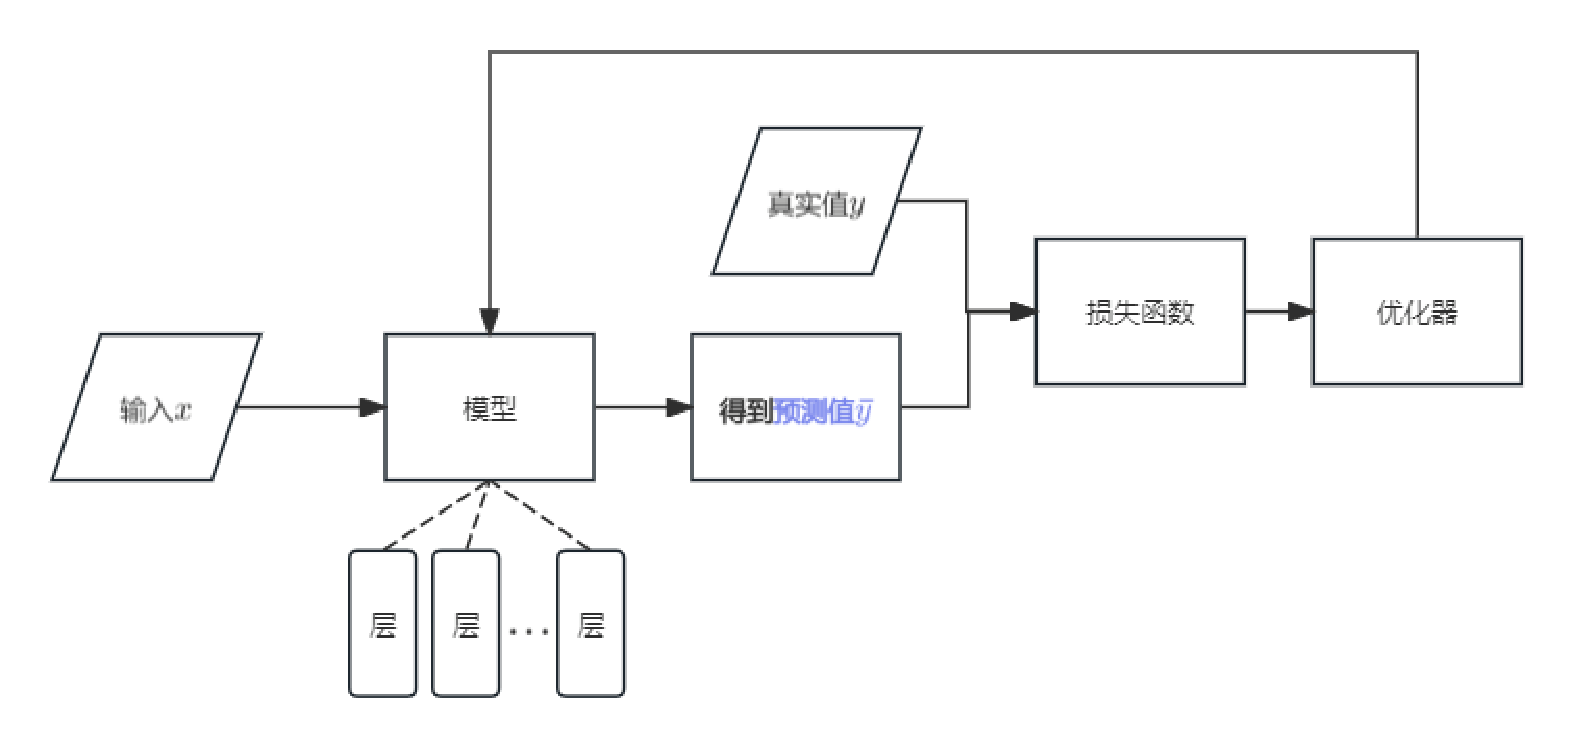
\includegraphics[width=0.8\textwidth]{part/人工智能/深度学习框架/pic/Pytorch/PyTorch神经网络工具/神经网络关键组件及相互关系示意图.pdf}
    \caption{神经网络关键组件及相互关系示意图}
    \label{fig:Pytorch_nn_core_components}
\end{figure}

如图\ref{fig:Pytorch_nn_core_components}所示，
多个层链接在一起构成一个模型或网络，输入数据通过这个模型转换为预测值。
预测值与真实值共同构成损失函数的输入，损失函数输出损失值（损失值可以是距离、概率值等），
该损失值用于衡量预测值与目标结果的匹配或相似程度。
优化器利用损失值更新权重参数，目标是使损失值越来越小。
这是一个循环过程，当损失值达到一个阈值或循环次数到达指定次数时，循环结束。


\section{构建神经网络的主要工具}
\subsection{nn.Module}
使用autograd及Tensor实现机器学习实例时，需要做不少设置，
如将叶子节点的参数\codeinline{requires\_grad}设置为\codeinline{True},
然后调用\codeinline{backward}函数从grad属性中提取梯度。
对于大规模的网络，autograd太过于底层和烦琐。
为了简单、有效地解决这个问题，\codeinline{nn}是一个有效工具。 
它是专门为深度学习设计的一个模块，而\codeinline{nn.Module}是\codeinline{nn}的一个核心数据结构。
\codeinline{nn.Module}可以是神经网络的某个层，也可以是包含多层的神经网络。
在实际使用中，最常见的做法是继承\codeinline{nn.Module}生成自己的网络层，

\codeinline{nn.Module}是PyTorch中所有神经网络模块的基类，
所有神经网络模块都应该继承自\codeinline{nn.Module}。

\subsection{nn.functional}
\label{subsubsec:Pytorch_nn_functional}
\codeinline{nn.functional}是一个函数模块，包含了神经网络中的一些常用函数，
如激活函数、损失函数、池化函数等。


\subsubsection{nn.Module和nn.functional的区别}
\label{subsubsec:Pytorch_nn_Module_and_nn_functional_difference}
\codeinline{nn}中的层，
\begin{enumerate}[label=\arabic*)]
    \item 继承了 \codeinline{nn.Module}，名称一般为\codeinline{nn.Xxx}(第一个是大写)

    如\codeinline{nn.Linear}、\codeinline{nn.Conv2d}、\codeinline{nn.CrossEntropyLoss} 等。

    \item  \codeinline{nn.functional} 中的函数，名称一般为 \codeinline{nn.functional.xxx}(第一个是小写)，

    如\codeinline{nn.functional.linear}、\codeinline{nn.functional.conv2d}、
 \codeinline{nn.functional.cross\_entropy} 等。
\end{enumerate}
 
  
从功能方面来说两者相当，基于\codeinline{nn.Module}实现的层，也可以基于\codeinline{nn.functional} 实现，反之亦然。
从性能方面来说两者也没有太大差异。不过在具体使用时，两者还是有区别的

\begin{enumerate}[label=\arabic*)]
    \item \codeinline{nn.Xxx}继承于\codeinline{nn.Module},需要先实例化并传入参数，
    然后以函数调用的方式调用实例化的对象并传入输入数据。它能够很好地与\codeinline{nn.Sequential}结合使用

    而\codeinline{nn.functional.xxx}是一个函数。它无法保存参数，因此无法使用\codeinline{nn.Sequential}。
    \item \codeinline{nn.Xxx}中的层可以\textcolor{YBXPurple}{自动}定义、保存参数，如\codeinline{nn.Linear}中的权重和偏置，

    而\codeinline{nn.functional.xxx}中的函数不具备保存参数的功能，不仅需要自己定义参数(权重(weights)和偏置(bias)等)，还需要手动传入参数。

    \item \codeinline{dropout}操作在训练和测试阶段是不同的，
    使用\codeinline{nn.Xxx}方式定义的\codeinline{dropout}层，在调用\codeinline{model.eval()}后，自动实现状态的转换，

    而使用\codeinline{nn.functional.xxx}方式定义的\codeinline{dropout}函数，需要手动设置状态。
\end{enumerate}

总的来说，两种函数的功能都是相同的，但PyTorch官方推荐：
\begin{enumerate}[label=\arabic*)]
    \item 具有学习参数的
    （例如，conv2d、linear、batchjnorm、dropout等）情况采用\codeinline{nn.Xxx}方式，
    \item 没有学习参数的
    （例如， maxpool, loss func, activation fimc 等）情况采用 \codeinline{nn.functional.xxx} 或者 \codeinline{nn.Xxx} 方式。
\end{enumerate}

\begin{lstlisting}[style=pythonstyle]
# 使用 nn.Module 定义一个简单的神经网络    
import torch
import torch.nn as nn
import torch.optim as optim

# 定义一个简单的神经网络，继承自 nn.Module
class Net(nn.Module):
    def __init__(self):
        super(Net, self).__init__()
        # 使用 nn.Xxx 自动定义和保存参数
        self.fc1 = nn.Linear(10, 20)
        self.fc2 = nn.Linear(20, 10)
        self.dropout = nn.Dropout(p=0.5)  # 定义 Dropout 层

    def forward(self, x):
        x = self.fc1(x)
        x = self.dropout(x)
        x = self.fc2(x)
        return x

# 使用 nn.Sequential 结合多层
net = nn.Sequential(
    nn.Linear(10, 20),
    nn.ReLU(),
    nn.Dropout(p=0.5),
    nn.Linear(20, 10)
)

# 打印 Dropout 在训练模式下的状态
print("Training mode:")
print(net)

# 创建一个随机输入张量
input_data = torch.randn(5, 10)

# 模型实例化并调用
model = Net()
output = model(input_data)

# 切换到 eval 模式，Dropout 状态将自动切换
print("Dropout before eval:", model.dropout.training)
model.eval()
print("Eval mode:")
print(model)

# 在训练和测试模式下输出模型的 Dropout 状况
model.eval()  # 切换到评估模式
print("Dropout after eval:", model.dropout.training)

# 训练优化器设置
optimizer = optim.SGD(model.parameters(), lr=0.01)
\end{lstlisting}
\begin{lstlisting}[style=demostyle,numbers=none] 
Training mode:
Sequential(
  (0): Linear(in_features=10, out_features=20, bias=True)
  (1): ReLU()
  (2): Dropout(p=0.5, inplace=False)
  (3): Linear(in_features=20, out_features=10, bias=True)
)
Dropout before eval: True
Eval mode:
Net(
  (fc1): Linear(in_features=10, out_features=20, bias=True)
  (fc2): Linear(in_features=20, out_features=10, bias=True)
  (dropout): Dropout(p=0.5, inplace=False)
)
Dropout after eval: False    
\end{lstlisting}
\begin{lstlisting}[style=pythonstyle]
# 使用 nn.functional 定义一个简单的神经网络
import torch
import torch.nn.functional as F

# 自定义一个简单的神经网络，不继承 nn.Module
class FunctionalNet:
    def __init__(self):
        # 手动定义权重和偏置
        self.weight1 = torch.randn(20, 10, requires_grad=True)
        self.bias1 = torch.randn(20, requires_grad=True)
        self.weight2 = torch.randn(10, 20, requires_grad=True)
        self.bias2 = torch.randn(10, requires_grad=True)
        self.dropout_p = 0.5
        self.training = True

    def forward(self, x):
        x = F.linear(x, self.weight1, self.bias1)
        if self.training:  # 手动设置 dropout 状态
            x = F.dropout(x, p=self.dropout_p)
        x = F.linear(x, self.weight2, self.bias2)
        return x

    def eval(self):
        self.training = False  # 手动切换为评估模式

# 实例化模型并传入输入数据
model = FunctionalNet()
input_data = torch.randn(5, 10)

# 模型训练模式下
print("Training mode")
output = model.forward(input_data)

# 手动切换到评估模式，关闭 dropout
print("Dropout before eval:", model.training)
model.eval()
print("Eval mode")
print("Dropout after eval:", model.training)
output = model.forward(input_data)

# 手动更新权重（这里只是为了演示，通常在训练步骤中会通过优化器更新）
optimizer = optim.SGD([model.weight1, model.bias1, model.weight2, model.bias2], lr=0.01)
\end{lstlisting}
\begin{lstlisting}[style=demostyle,numbers=none] 
Training mode
Dropout before eval: True
Eval mode
Dropout after eval: False
\end{lstlisting}    


\section{构建模型的方法}
\label{subsec:Pytorch_build_model}
使用PyTorch构建模型的方法大致有以下3种。
\begin{enumerate}[label=\arabic*)]
    \item 继承\codeinline{nn.Module}基类构建模型。
    \item 使用\codeinline{nn.Sequential}按层顺序构建模型。
    \item 继承\codeinline{nn.Module}基类构建模型，再使用相关模型容器（如\codeinline{nn.Sequential}、\codeinline{nn.ModuleList}、\codeinline{nn.ModuleDict}等）进行封装。
\end{enumerate}

\begin{example}
    \exProblem
    如图\ref{fig:Pytorch_build_model_example}所示，使用PyTorch构建一个简单的神经网络模型，使用3种方法构建模型。
    \begin{figure}[htpb]
        \centering
        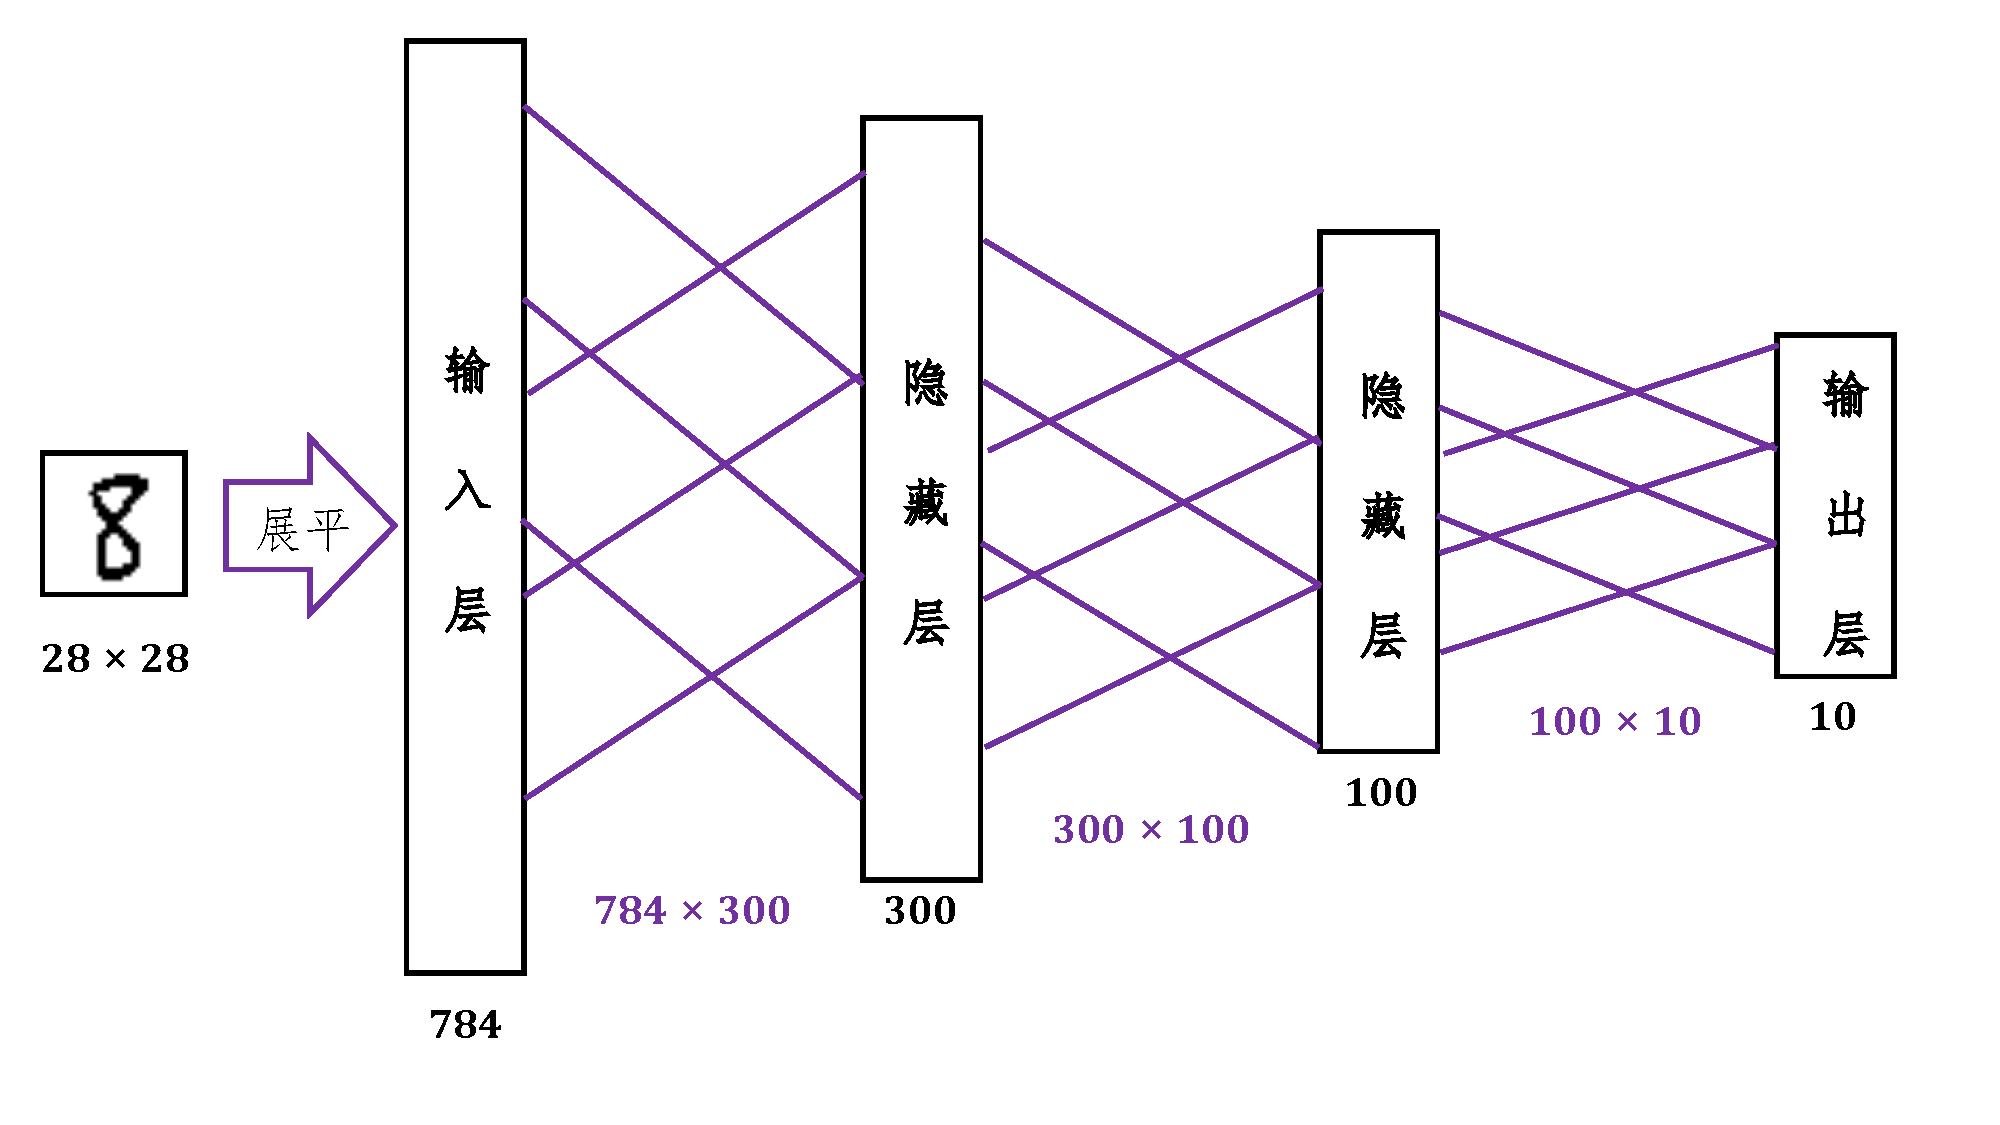
\includegraphics[width=0.8\textwidth]{part/人工智能/深度学习框架/pic/Pytorch/PyTorch神经网络工具/使用PyTorch构建模型的演示.pdf}
        \caption{使用PyTorch构建模型的演示}
        \label{fig:Pytorch_build_model_example}
    \end{figure}
    
\end{example}


\subsection{继承nn.Module基类构建模型}
\label{subsubsec:Pytorch_build_model_inherit_nn_Module}
利用这种方法构建模型，先定义一个类，使之继承\codeinline{nn.Module}基类。
把模型中需要用到的层放在构造函数\codeinline{\_\_init\_\_()}中，
在\codeinline{forward}方法中实现模型的正向传播。

\begin{lstlisting}[style=pythonstyle]
# 构建神经网络 
# 方法1.继承 nn.Module 类
import torch
from torch import nn # 导入nn 模块
import torch.nn.functional as F # 导入函数模块

###########################
class Model(nn.Module):
    def __init__(self, in_dim, n_hidden_1, n_hidden_2, out_dim):
        super(Model, self).__init__()
        self.layer1 = nn.Linear(in_dim, n_hidden_1)
        self.layer2 = nn.Linear(n_hidden_1, n_hidden_2)
        self.layer3 = nn.Linear(n_hidden_2, out_dim)

    def forward(self, x):
        x = F.relu(self.layer1(x))
        x = F.relu(self.layer2(x))
        x = self.layer3(x)
        return x
    
## 实例化模型
model = Model(10, 20, 10, 6) # 输入是10，输出是6
print(model)

x = torch.randn(10) # 这里是10
print("x:", x)
print(model.forward(x))
\end{lstlisting}
\begin{lstlisting}[style=demostyle,numbers=none] 
Model(
  (layer1): Linear(in_features=10, out_features=20, bias=True)
  (layer2): Linear(in_features=20, out_features=10, bias=True)
  (layer3): Linear(in_features=10, out_features=6, bias=True)
)
x: tensor([-1.0035,  0.4780,  0.8982,  0.0782, -1.2985, -0.5568,  0.2565,  1.2554,
         0.1004,  0.4208])
tensor([-0.0519,  0.0176,  0.0493, -0.2996, -0.1996,  0.1357], # 输出层是6个神经元
       grad_fn=<ViewBackward0>)
\end{lstlisting}

\begin{lstlisting}[style=pythonstyle]
# 导入模块
import torch
from torch import nn            # 导入 nn 模块
import torch.nn.functional as F # 导入函数模块

################################
# 构建模型
class Model_inh_mod(nn.Module): # 通过继承 nn.Module 来构建模型
    def __init__(self, in_dim, n_hidden_1, n_hidden_2, out_dim):
        super(Model_use_Seq, self).__init__()
        self.flatten = nn.Flatten() # 展平操作
        self.linear1 = nn.Linear(in_dim, n_hidden_1)
        self.bn1 = nn.BatchNorm1d(n_hidden_1) # 批量归一化
        self.linear2 = nn.Linear(n_hidden_1, n_hidden_2)
        self.bn2 = nn.BatchNorm1d(n_hidden_2)
        self.out = nn.Linear(n_hidden_2, out_dim)

    def forward(self, x):
        x = self.flatten(x)
        x = self.linear1(x)
        x = self.bn1(x)
        x = F.relu(x)
        x = self.linear2(x)
        x = self.bn2(x)
        x = F.relu(x)
        x = self.out(x)
        x = F.softmax(x, dim=1)
        return x

# 查看模型    
# 定义一个28*28的输入，
# 第一个隐藏层300个神经元，第二个隐藏层100个神经元，
# 输出层10个神经元
in_dim, n_hidden_1, n_hidden_2, out_dim = 28*28, 300, 100, 10
model = Model_inh_mod(in_dim, n_hidden_1, n_hidden_2, out_dim)
print(model)
\end{lstlisting}
\begin{lstlisting}[style=demostyle,numbers=none]
Model_inh_mod(
  (flatten): Flatten(start_dim=1, end_dim=-1)
  (linear1): Linear(in_features=784, out_features=300, bias=True)
  (bn1): BatchNorm1d(300, eps=1e-05, momentum=0.1, affine=True, track_running_stats=True)
  (linear2): Linear(in_features=300, out_features=100, bias=True)
  (bn2): BatchNorm1d(100, eps=1e-05, momentum=0.1, affine=True, track_running_stats=True)
  (out): Linear(in_features=100, out_features=10, bias=True)
)    
\end{lstlisting}


\subsection{使用nn.Sequential按层顺序构建模型}
\label{subsubsec:Pytorch_build_model_with_nn_Sequential}
\begin{enumerate}[label=\arabic*)]
    \item 利用可变参数
    Python中的函数的参数个数是可变(或称为不定长参数)的，
    PyTorch中的有些函数也与此类似，\codeinline{nn.Sequential(*args)}。
    \begin{lstlisting}[style=pythonstyle]
    # 方法2 使用nn.Sequential
    import torch
    from torch import nn

    # 定义模型
    in_dim, n_hidden_1, n_hidden_2, out_dim = 10, 20, 10, 6

    model = nn.Sequential(
        nn.Linear(in_dim, n_hidden_1),
        nn.ReLU(),
        nn.Linear(n_hidden_1, n_hidden_2),
        nn.ReLU(),
        nn.Linear(n_hidden_2, out_dim)
    )

    # 打印模型
    print(model)

    # 测试模型
    x = torch.tensor([1, 2, 3, 4, 5, 6, 7, 8, 9, 10], dtype=torch.float32)
    print("x:", x)
    print(model(x))
    \end{lstlisting}

\begin{lstlisting}[style=pythonstyle]
# 导入模块
import torch
from torch import nn            # 导入 nn 模块
# 初始化参数
in_dim, n_hidden_1, n_hidden_2, out_dim = 28*28, 300, 100, 10

################################
# 构建模型
Model_use_Seq = nn.Sequential(
    nn.Flatten(), # 展平操作
    nn.Linear(in_dim, n_hidden_1),
    nn.BatchNorm1d(n_hidden_1), # 批量归一化
    nn.ReLU(),
    nn.Linear(n_hidden_1, n_hidden_2),
    nn.BatchNorm1d(n_hidden_2),
    nn.ReLU(),
    nn.Linear(n_hidden_2, out_dim),
    nn.Softmax(dim=1)
    )

# 查看模型
model = Model_use_Seq
print(model)
\end{lstlisting}
\begin{lstlisting}[style=demostyle,numbers=none]
Sequential(
  (0): Flatten(start_dim=1, end_dim=-1)
  (1): Linear(in_features=784, out_features=300, bias=True)
  (2): BatchNorm1d(300, eps=1e-05, momentum=0.1, affine=True, track_running_stats=True)
  (3): ReLU()
  (4): Linear(in_features=300, out_features=100, bias=True)
  (5): BatchNorm1d(100, eps=1e-05, momentum=0.1, affine=True, track_running_stats=True)
  (6): ReLU()
  (7): Linear(in_features=100, out_features=10, bias=True)
  (8): Softmax(dim=1)
)
\end{lstlisting}   
    
    \item 使用\codeinline{add\_module}方法
\begin{lstlisting}[style=pythonstyle]
# 导入模块
import torch
from torch import nn            # 导入 nn 模块
# 初始化参数
in_dim, n_hidden_1, n_hidden_2, out_dim = 28*28, 300, 100, 10

################################
# 构建模型
Seq_model = nn.Sequential()
Seq_model.add_module('flatten', nn.Flatten())
Seq_model.add_module('linear1', nn.Linear(in_dim, n_hidden_1))
Seq_model.add_module('bn1', nn.BatchNorm1d(n_hidden_1))
Seq_model.add_module('relu1', nn.ReLU())
Seq_model.add_module('linear2', nn.Linear(n_hidden_1, n_hidden_2))
Seq_model.add_module('bn2', nn.BatchNorm1d(n_hidden_2))
Seq_model.add_module('relu2', nn.ReLU())
Seq_model.add_module('out', nn.Linear(n_hidden_2, out_dim))
Seq_model.add_module('softmax', nn.Softmax(dim=1))

# 查看模型
model = Seq_model
print(model)
\end{lstlisting}
\begin{lstlisting}[style=demostyle,numbers=none]
Sequential(
  (flatten): Flatten(start_dim=1, end_dim=-1)
  (linear1): Linear(in_features=784, out_features=300, bias=True)
  (bn1): BatchNorm1d(300, eps=1e-05, momentum=0.1, affine=True, track_running_stats=True)
  (relu1): ReLU()
  (linear2): Linear(in_features=300, out_features=100, bias=True)
  (bn2): BatchNorm1d(100, eps=1e-05, momentum=0.1, affine=True, track_running_stats=True)
  (relu2): ReLU()
  (out): Linear(in_features=100, out_features=10, bias=True)
  (softmax): Softmax(dim=1)
)
\end{lstlisting}

    \item 使用\codeinline{OrderedDict}方法
\begin{lstlisting}[style=pythonstyle]
# 导入模块
import torch
from torch import nn            # 导入 nn 模块
from collections import OrderedDict

# 初始化参数
in_dim, n_hidden_1, n_hidden_2, out_dim = 28*28, 300, 100, 10

################################
# 构建模型
Seq_model = nn.Sequential(OrderedDict([
    ('flatten', nn.Flatten()),
    ('linear1', nn.Linear(in_dim, n_hidden_1)),
    ('bn1', nn.BatchNorm1d(n_hidden_1)),
    ('relu1', nn.ReLU()),
    ('linear2', nn.Linear(n_hidden_1, n_hidden_2)),
    ('bn2', nn.BatchNorm1d(n_hidden_2)),
    ('relu2', nn.ReLU()),
    ('out', nn.Linear(n_hidden_2, out_dim)),
    ('softmax', nn.Softmax(dim=1))
    ]))

# 查看模型
model = Seq_model
print(model)    
\end{lstlisting}
\begin{lstlisting}[style=demostyle,numbers=none]
Sequential(
  (flatten): Flatten(start_dim=1, end_dim=-1)
  (linear1): Linear(in_features=784, out_features=300, bias=True)
  (bn1): BatchNorm1d(300, eps=1e-05, momentum=0.1, affine=True, track_running_stats=True)
  (relu1): ReLU()
  (linear2): Linear(in_features=300, out_features=100, bias=True)
  (bn2): BatchNorm1d(100, eps=1e-05, momentum=0.1, affine=True, track_running_stats=True)
  (relu2): ReLU()
  (out): Linear(in_features=100, out_features=10, bias=True)
  (softmax): Softmax(dim=1)
)
\end{lstlisting}    


\end{enumerate}

\subsection{继承nn.Module基类构建模型，再使用相关模型容器进行封装}
\label{subsubsec:Pytorch_build_model_with_nn_Module_container}
\begin{enumerate}[label=\arabic*)]
    \item 使用\codeinline{nn.Sequential}封装
\begin{lstlisting}[style=pythonstyle]
# 导入模块
import torch
from torch import nn            # 导入 nn 模块
import torch.nn.functional as F # 导入函数模块

################################
# 构建模型
class Model_use_Seq(nn.Module): # 通过继承 nn.Module 来构建模型
    def __init__(self, in_dim, n_hidden_1, n_hidden_2, out_dim):
        super(Model_use_Seq, self).__init__()
        self.flatten = nn.Flatten() # 展平操作
        self.layer1 = nn.Sequential(nn.Linear(in_dim, n_hidden_1), nn.BatchNorm1d(n_hidden_1)) # 线性层和批量归一化层
        self.layer2 = nn.Sequential(nn.Linear(n_hidden_1, n_hidden_2), nn.BatchNorm1d(n_hidden_2))
        self.out = nn.Linear(n_hidden_2, out_dim)

    def forward(self, x):
        x = self.flatten(x)
        x = F.relu(self.layer1(x))
        x = F.relu(self.layer2(x))
        x = F.softmax(self.out(x), dim=1)
        return x
    
# 查看模型
# 定义一个28*28的输入，
# 第一个隐藏层300个神经元，第二个隐藏层100个神经元，
# 输出层10个神经元
in_dim, n_hidden_1, n_hidden_2, out_dim = 28*28, 300, 100, 10
model = Model_use_Seq(in_dim, n_hidden_1, n_hidden_2, out_dim)
print(model)
\end{lstlisting}
\begin{lstlisting}[style=demostyle,numbers=none]
Model_use_Seq(
  (flatten): Flatten(start_dim=1, end_dim=-1)
  (layer1): Sequential(
    (0): Linear(in_features=784, out_features=300, bias=True)
    (1): BatchNorm1d(300, eps=1e-05, momentum=0.1, affine=True, track_running_stats=True)
  )
  (layer2): Sequential(
    (0): Linear(in_features=300, out_features=100, bias=True)
    (1): BatchNorm1d(100, eps=1e-05, momentum=0.1, affine=True, track_running_stats=True)
  )
  (out): Linear(in_features=100, out_features=10, bias=True)
)    
\end{lstlisting}

    \item 使用\codeinline{nn.ModuleList}封装
\begin{lstlisting}[style=pythonstyle]
# 导入模块
import torch
from torch import nn            # 导入 nn 模块
import torch.nn.functional as F # 导入函数模块

################################
# 构建模型
class Model_use_modlist(nn.Module): # 通过继承 nn.Module 来构建模型
    def __init__(self, in_dim, n_hidden_1, n_hidden_2, out_dim):
        super(Model_use_modlist, self).__init__()
        self.layers = nn.ModuleList([nn.Flatten(), 
                                     nn.Linear(in_dim, n_hidden_1),
                                     nn.BatchNorm1d(n_hidden_1),
                                     nn.ReLU(),
                                     nn.Linear(n_hidden_1, n_hidden_2),
                                     nn.BatchNorm1d(n_hidden_2),
                                     nn.ReLU(),
                                     nn.Linear(n_hidden_2, out_dim),
                                     nn.Softmax(dim=1)])

    def forward(self, x):
        for layer in self.layers:
            x = layer(x)
        return x

# 查看模型
# 定义一个28*28的输入，
# 第一个隐藏层300个神经元，第二个隐藏层100个神经元，
# 输出层10个神经元
in_dim, n_hidden_1, n_hidden_2, out_dim = 28*28, 300, 100, 10
model = Model_use_modlist(in_dim, n_hidden_1, n_hidden_2, out_dim)
print(model)    
\end{lstlisting}
\begin{lstlisting}[style=demostyle,numbers=none]
Model_use_modlist(
  (layers): ModuleList(
    (0): Flatten(start_dim=1, end_dim=-1)
    (1): Linear(in_features=784, out_features=300, bias=True)
    (2): BatchNorm1d(300, eps=1e-05, momentum=0.1, affine=True, track_running_stats=True)
    (3): ReLU()
    (4): Linear(in_features=300, out_features=100, bias=True)
    (5): BatchNorm1d(100, eps=1e-05, momentum=0.1, affine=True, track_running_stats=True)
    (6): ReLU()
    (7): Linear(in_features=100, out_features=10, bias=True)
    (8): Softmax(dim=1)
  )
)
\end{lstlisting}

    \item 使用\codeinline{nn.ModuleDict}封装
\begin{lstlisting}[style=pythonstyle]
# 导入模块
import torch
from torch import nn            # 导入 nn 模块

################################
# 构建模型
class Model_use_dict(nn.Module): # 通过继承 nn.Module 来构建模型
    def __init__(self, in_dim, n_hidden_1, n_hidden_2, out_dim):
        super(Model_use_dict, self).__init__()
        self.layers = nn.ModuleDict({
            'flatten': nn.Flatten(),
            'linear1': nn.Linear(in_dim, n_hidden_1),
            'bn1': nn.BatchNorm1d(n_hidden_1),
            'relu1': nn.ReLU(),
            'linear2': nn.Linear(n_hidden_1, n_hidden_2),
            'bn2': nn.BatchNorm1d(n_hidden_2),
            'relu2': nn.ReLU(),
            'out': nn.Linear(n_hidden_2, out_dim),
            'softmax': nn.Softmax(dim=1)
        })

    def forward(self, x):
        for layer in self.layers.values():
            x = layer(x)
        return x
    
# 查看模型
in_dim, n_hidden_1, n_hidden_2, out_dim = 28*28, 300, 100, 10
model = Model_use_dict(in_dim, n_hidden_1, n_hidden_2, out_dim)
print(model)    
\end{lstlisting}
其中激活函数ReLU在模型中应该出现2次，
但在定义字典时，只需定义一次，
在定义forward函数的列表中则需要出现2次。

\begin{lstlisting}[style=demostyle,numbers=none]
Model_use_dict(
  (layers): ModuleDict(
    (flatten): Flatten(start_dim=1, end_dim=-1)
    (linear1): Linear(in_features=784, out_features=300, bias=True)
    (bn1): BatchNorm1d(300, eps=1e-05, momentum=0.1, affine=True, track_running_stats=True)
    (relu1): ReLU()
    (linear2): Linear(in_features=300, out_features=100, bias=True)
    (bn2): BatchNorm1d(100, eps=1e-05, momentum=0.1, affine=True, track_running_stats=True)
    (relu2): ReLU()
    (out): Linear(in_features=100, out_features=10, bias=True)
    (softmax): Softmax(dim=1)
  )
)
\end{lstlisting}            
\end{enumerate}

\section{损失优化}
\label{subsec:Pytorch_loss_optimization}
\subsection{Pytorch激活函数}
\label{subsubsec:Pytorch_nn_functional_activation_function}
第\pageref{subsubsec:激活函数}页激活函数一节中介绍了常见的激活函数，
PyTorch中也提供了这些激活函数，如表\ref{tab:Pytorch_Activation_Expressions}所示。

\begin{table}[h]
\centering
\resizebox{0.8\textwidth}{!}{
    \begin{tabular}{|l|c|l|}
        \hline
        \textbf{激活函数} & \textbf{表达式} & \textbf{调用方法} \\ \hline
        nn.Sigmoid & $\text{Sigmoid}(x) = \frac{1}{1 + \exp(-x)}$ & torch.nn.Sigmoid() \\ \hline
        nn.Tanh & $\text{Tanh}(x) = \frac{\exp(x) - \exp(-x)}{\exp(x) + \exp(-x)}$ & torch.nn.Tanh() \\ \hline
        nn.ReLU & $\text{ReLU}(x) = \max(0, x)$ & torch.nn.ReLU(inplace=False) \\ \hline
        nn.LeakyReLU & $\text{LeakyReLU}(x) = \begin{cases} x, & \text{if } x \geq 0 \\ \text{negative\_slope} \cdot x, & \text{if } x < 0 \end{cases}$ & torch.nn.LeakyReLU(negative\_slope=0.01, inplace=False) \\ \hline
        nn.ELU & $\text{ELU}(x) = \begin{cases} x, & \text{if } x > 0 \\ \alpha (\exp(x) - 1), & \text{if } x \leq 0 \end{cases}$ & torch.nn.ELU(alpha=1.0, inplace=False) \\ \hline
        nn.Hardshrink & $\text{Hardshrink}(x) = \begin{cases} x, & \text{if } |x| > \lambda \\ 0, & \text{if } |x| \leq \lambda \end{cases}$ & torch.nn.Hardshrink(lambd=0.5) \\ \hline
        nn.Hardsigmoid & $\text{Hardsigmoid}(x) = \max(0, \min(1, \frac{x+1}{2}))$ & torch.nn.Hardsigmoid(inplace=False) \\ \hline
        nn.Hardtanh & $\text{Hardtanh}(x) = \begin{cases} 1, & \text{if } x > 1 \\ -1, & \text{if } x < -1 \\ x, & \text{otherwise} \end{cases}$ & torch.nn.Hardtanh(min\_val=-1.0, max\_val=1.0) \\ \hline
        nn.Hardswish & $\text{Hardswish}(x) = x \cdot \frac{\min(\max(x + 3, 0), 6)}{6}$ & torch.nn.Hardswish(inplace=False) \\ \hline
        nn.LogSigmoid & $\text{LogSigmoid}(x) = \log(\frac{1}{1 + \exp(-x)})$ & torch.nn.LogSigmoid() \\ \hline
        nn.MultiheadAttention & - & torch.nn.MultiheadAttention(embed\_dim, num\_heads, ...) \\ \hline
        nn.PReLU & $\text{PReLU}(x) = \begin{cases} x, & \text{if } x \geq 0 \\ a \cdot x, & \text{if } x < 0 \end{cases}$ & torch.nn.PReLU(num\_parameters=1, init=0.25) \\ \hline
        nn.ReLU6 & $\text{ReLU6}(x) = \min(\max(0, x), 6)$ & torch.nn.ReLU6(inplace=False) \\ \hline
        nn.RReLU & $\text{RReLU}(x) = \begin{cases} x, & \text{if } x \geq 0 \\ a \cdot x, & \text{if } x < 0 \end{cases}$ & torch.nn.RReLU(lower=0.125, upper=0.33, inplace=False) \\ \hline
        nn.SELU & $\text{SELU}(x) = \lambda \cdot \begin{cases} x, & \text{if } x > 0 \\ \alpha \cdot (\exp(x) - 1), & \text{if } x \leq 0 \end{cases}$ & torch.nn.SELU(inplace=False) \\ \hline
        nn.CELU & $\text{CELU}(x) = \begin{cases} x, & \text{if } x > 0 \\ \alpha (\exp(\frac{x}{\alpha}) - 1), & \text{if } x \leq 0 \end{cases}$ & torch.nn.CELU(alpha=1.0, inplace=False) \\ \hline
        nn.GELU & $\text{GELU}(x) = 0.5 \cdot x \cdot \left[1 + \tanh(\sqrt{\frac{2}{\pi}} (x + 0.044715 \cdot x^3))\right]$ & torch.nn.GELU() \\ \hline
        nn.SiLU & $\text{SiLU}(x) = \frac{x}{1 + \exp(-x)}$ & torch.nn.SiLU(inplace=False) \\ \hline
        nn.Softplus & $\text{Softplus}(x) = \frac{1}{\beta} \log(1 + \exp(\beta x))$ & torch.nn.Softplus(beta=1, threshold=20) \\ \hline
        nn.Softshrink & $\text{Softshrink}(x) = \begin{cases} x - \lambda, & \text{if } x > \lambda \\ x + \lambda, & \text{if } x < -\lambda \\ 0, & \text{otherwise} \end{cases}$ & torch.nn.Softshrink(lambd=0.5) \\ \hline
        nn.Softsign & $\text{Softsign}(x) = \frac{x}{1 + |x|}$ & torch.nn.Softsign() \\ \hline
        nn.Tanhshrink & $\text{Tanhshrink}(x) = x - \tanh(x)$ & torch.nn.Tanhshrink() \\ \hline
        nn.Threshold & $\text{Threshold}(x) = \begin{cases} x, & \text{if } x > \text{threshold} \\ \text{value}, & \text{if } x \leq \text{threshold} \end{cases}$ & torch.nn.Threshold(threshold, value, inplace=False) \\ \hline
        nn.Softmin & $\text{Softmin}(x_i) = \frac{\exp(-x_i)}{\sum_j \exp(-x_j)}$ & torch.nn.Softmin(dim=None) \\ \hline
        nn.Softmax & $\text{Softmax}(x_i) = \frac{\exp(x_i)}{\sum_j \exp(x_j)}$ & torch.nn.Softmax(dim=None) \\ \hline
        nn.Softmax2d & - & torch.nn.Softmax2d() \\ \hline
        nn.LogSoftmax & $\text{LogSoftmax}(x_i) = \log\left(\frac{\exp(x_i)}{\sum_j \exp(x_j)}\right)$ & torch.nn.LogSoftmax(dim=None) \\ \hline
        nn.AdaptiveLogSoftmaxWithLoss & - & torch.nn.AdaptiveLogSoftmaxWithLoss(...) \\ \hline
    \end{tabular}
}
\caption{PyTorch激活函数及其表达式和调用方法}
\label{tab:Pytorch_Activation_Expressions}
\end{table}

\subsection{Pytorch损失函数}
\label{subsubsec:Pytorch_nn_functional_loss_function}
第\pageref{subsec:误差函数}页误差函数一节中介绍了常见的损失函数，主要出现在反向传播中，
如表\ref{tab:Pytorch_Loss_Functions_Detailed}所示，就是PyTorch中的损失函数。

\begin{table}[h]
\centering
\resizebox{0.9\textwidth}{!}{
    \begin{tabular}{|l|l|l|l|}
        \hline
        \textbf{损失函数} & \textbf{函数说明} & \textbf{表达式} & \textbf{调用方法} \\ \hline
        nn.L1Loss & L1 范数损失函数 & $\text{L1Loss}(x) = \sum |x_i - y_i|$ & torch.nn.L1Loss(size\_average=None, reduce=None, reduction='mean') \\ \hline
        nn.MSELoss & 均方误差损失函数 & $\text{MSELoss}(x) = \frac{1}{n} \sum (x_i - y_i)^2$ & torch.nn.MSELoss(reduce=True, size\_average=True, reduction='mean') \\ \hline
        nn.CrossEntropyLoss & 交叉熵损失函数 & $\text{CrossEntropyLoss}(x) = -\sum y_i \log(p(x_i))$ & torch.nn.CrossEntropyLoss(weight=None, size\_average=None, ignore\_index=-100, reduce=None, reduction='mean') \\ \hline
        nn.CosineEmbeddingLoss & 余弦相似度损失函数 & $\begin{aligned}\left.\text{CosineEmbeddingLoss}(x, y)=\left\{\begin{matrix}1-\cos(x_1,x_2) ,&\quad y=1\\\max(0,\cos(x_1,x_2)-margin) ,&\quad y=-1\end{matrix}\right.\right.\end{aligned}$ & torch.nn.CosineEmbeddingLoss(margin=0.0, reduction='mean') \\ \hline
        nn.CTCLoss & 连接时序分类损失 & - & torch.nn.CTCLoss() \\ \hline
        nn.NLLLoss & 负对数似然损失 & $\text{NLLLoss}(x) = -\sum y_i \log(p(x_i))$ & torch.nn.NLLLoss() \\ \hline
        nn.PoissonNLLLoss & 泊松负对数似然损失 & $\text{PoissonNLLLoss}(x) = \log(\frac{(y - x)}{y!})$ & torch.nn.PoissonNLLLoss() \\ \hline
        nn.GaussianNLLLoss & 高斯负对数似然损失 & $\text{GaussianNLLLoss}(x) = \frac{1}{2} \log(2\pi \sigma^2) + \frac{(x - \mu)^2}{2\sigma^2}$ & torch.nn.GaussianNLLLoss() \\ \hline
        nn.KLDivLoss & KL 散度损失 & $D_{KL}(P || Q) = \sum P(x) \log(\frac{P(x)}{Q(x)})$ & torch.nn.KLDivLoss() \\ \hline
        nn.BCELoss & 二进制交叉熵损失 & $\text{BCELoss}(x) = - \sum y \log(p(x)) + (1-y) \log(1-p(x))$ & torch.nn.BCELoss() \\ \hline
        nn.BCEWithLogitsLoss & 逻辑二进制交叉熵损失 & - & torch.nn.BCEWithLogitsLoss() \\ \hline
        nn.MarginRankingLoss & 间隔排序损失 & $\text{MarginRankingLoss}(x) = \max(0, -y (x_1 - x_2) + \text{margin})$ & torch.nn.MarginRankingLoss() \\ \hline
        nn.HingeEmbeddingLoss & 铰链嵌入损失 & $\text{HingeEmbeddingLoss}(x) = \max(0, 1 - yx)$ & torch.nn.HingeEmbeddingLoss() \\ \hline
        nn.MultiLabelMarginLoss & 多标签分类损失 & - & torch.nn.MultiLabelMarginLoss() \\ \hline
        nn.SoftMarginLoss & 两分类逻辑损失 & - & torch.nn.SoftMarginLoss() \\ \hline
        nn.MultiLabelSoftMarginLoss & 多标签逻辑损失 & - & torch.nn.MultiLabelSoftMarginLoss() \\ \hline
        nn.SmoothL1Loss & 平滑 L1 损失 & $\text{SmoothL1Loss}(x) = \begin{cases} 0.5 (x - y)^2, & \text{if } |x - y| < 1 \\ |x - y| - 0.5, & \text{otherwise} \end{cases}$ & torch.nn.SmoothL1Loss() \\ \hline
        nn.MultiMarginLoss & 多类别分类损失 & - & torch.nn.MultiMarginLoss() \\ \hline
        nn.TripletMarginLoss & 三元组损失 & - & torch.nn.TripletMarginLoss() \\ \hline
        nn.TripletMarginWithDistanceLoss & 距离三元组损失 & - & torch.nn.TripletMarginWithDistanceLoss() \\ \hline
    \end{tabular}
}
\caption{损失函数及其函数说明、表达式和调用方法}
\label{tab:Pytorch_Loss_Functions_Detailed}
\end{table}

其中常用的
\begin{enumerate}[label=\arabic*)]
    \item L1 范数损失函数：\codeinline{nn.L1Loss}
    \begin{lstlisting}[style=demostyle,numbers=none] 
    loss = nn.L1Loss(size_average=False, reduce=False, reduction='mean')
    # size_average：当reduce=True时有效。
    #   为True时，返回的loss为平均值；
    #   为False时， 返回各样本的loss数值之和。
    # reduce:返回值是否为标量，默认为True。
    \end{lstlisting}
\begin{lstlisting}[style=pythonstyle]
import torch

# L1Loss 使用 reduction='mean'，即对所有样本的损失取均值
loss_mean = torch.nn.L1Loss(reduction='mean')
input = torch.tensor([1.0, 2.0, 6.0, 5.0])
target = torch.tensor([4.0, 5.0, 6.0, 7.0])
output_mean = loss_mean(input, target)
print(f"使用 reduction='mean' 的输出: {output_mean.item()}")  # 输出: 2.0

# L1Loss 使用 reduction='sum'，即对所有样本的损失取和
loss_sum = torch.nn.L1Loss(reduction='sum')
output_sum = loss_sum(input, target)
print(f"使用 reduction='sum' 的输出: {output_sum.item()}")  # 输出: 8.0

# L1Loss 使用 reduction='none'，即不对损失进行任何聚合
loss_none = torch.nn.L1Loss(reduction='none')
output_none = loss_none(input, target)
print(f"使用 reduction='none' 的输出: {output_none}")  # 输出: tensor([3., 3., 0., 2.])

###################################################
# 下面的方法在 PyTorch 1.0.0 版本后已经被废弃
# 使用 size_average 和 reduce 参数来模拟上述情况
# size_average=True, reduce=True 等效于 reduction='mean'
loss_size_average = torch.nn.L1Loss(size_average=True, reduce=True)
output_size_average = loss_size_average(input, target)
print(f"使用 size_average=True, reduce=True 的输出: {output_size_average.item()}")  # 输出: 2.0

# size_average=False, reduce=True 等效于 reduction='sum'
loss_reduce_sum = torch.nn.L1Loss(size_average=False, reduce=True)
output_reduce_sum = loss_reduce_sum(input, target)
print(f"使用 size_average=False, reduce=True 的输出: {output_reduce_sum.item()}")  # 输出: 8.0

# size_average=False, reduce=False 等效于 reduction='none'
loss_reduce_none = torch.nn.L1Loss(size_average=False, reduce=False)
output_reduce_none = loss_reduce_none(input, target)
print(f"使用 size_average=False, reduce=False 的输出: {output_reduce_none}")  # 输出: tensor([3., 3., 0., 2.])
\end{lstlisting}
\begin{lstlisting}[style=demostyle,numbers=none]
使用 reduction='mean' 的输出: 2.0
使用 reduction='sum' 的输出: 8.0
使用 reduction='none' 的输出: tensor([3., 3., 0., 2.])

###################################################
使用 size_average=True, reduce=True 的输出: 2.0
使用 size_average=False, reduce=True 的输出: 8.0
使用 size_average=False, reduce=False 的输出: tensor([3., 3., 0., 2.])    
\end{lstlisting}
\begin{example}
    \exProblem
    给定输入$input = [1.0, 2.0, 6.0, 5.0]$, 目标$target = [4.0, 5.0, 6.0, 7.0]$，计算L1范数损失函数。
    \exSolution
    L1损失函数('torch.nn.L1Loss’)的定义是目标值和预测值之间的绝对差值。数学公式如下：
    $$\mathrm{L1Loss}=\frac1N\sum_{i=1}^N|y_i-\hat{y}_i|$$
    其中：
    $y_i$是目标值。 $\hat{y}_i$是预测值。$N$是样本的数量。

    $|1.0 - 4.0|=3.0, |2.0 - 5.0|=3.0, |6.0 - 6.0|=0.0, |5.0 - 7.0|=2.0$，所以损失值为$[3.0, 3.0, 0.0, 2.0]$。

    \begin{enumerate}[label=\arabic*)]
        \item 当 \codeinline{reduction='mean'} 时：
        对损失进行平均，输出值为$output=\frac{3.0+3.0+0.0+2.0}{4}=2.0$。
        \item 当 \codeinline{reduction='sum'} 时：
        对损失进行求和，输出值为$output=3.0+3.0+0.0+2.0=8.0$。
        \item 当 \codeinline{reduction='none'} 时：
        不进行任何聚合操作，输出的张量为每个样本的绝对误差：\codeinline{tensor([3., 3., 0., 2.])}。
    \end{enumerate}
\end{example}


    \item 均方误差损失函数：\codeinline{nn.MSELoss}
    \begin{lstlisting}[style=demostyle,numbers=none] 
    loss = nn.MSELoss(reduce=False, size_average=False, reduction='mean')
    # size_average：当reduce=True时有效。
    #   为True时，返回的loss为平均值；
    #   为False时， 返回各样本的loss数值之和。
    # reduce:返回值是否为标量，默认为True。
    \end{lstlisting}
\begin{lstlisting}[style=pythonstyle]
import torch

# 使用 MSELoss (均方误差损失函数)
# reduction='mean': 对所有样本的平方误差取均值
loss_mse = torch.nn.MSELoss(reduction='mean')
input = torch.tensor([1.5, 3.0, 5.0, 4.0])
target = torch.tensor([4.0, 2.0, 6.0, 7.0])
output_mse = loss_mse(input, target)
print(f"使用 reduction='mean' 的 MSE 损失输出: {output_mse.item()}")  # 输出: 4.25

# 使用 MSELoss, reduction='sum'：对所有样本的平方误差取和
loss_mse_sum = torch.nn.MSELoss(reduction='sum')
output_mse_sum = loss_mse_sum(input, target)
print(f"使用 reduction='sum' 的 MSE 损失输出: {output_mse_sum.item()}")  # 输出: 17.0

# 使用 MSELoss, reduction='none'：不对损失进行任何聚合
loss_mse_none = torch.nn.MSELoss(reduction='none')
output_mse_none = loss_mse_none(input, target)
print(f"使用 reduction='none' 的 MSE 损失输出: {output_mse_none}")  # 输出: tensor([6.25, 1.00, 1.00, 8.75])
\end{lstlisting}
\begin{lstlisting}[style=demostyle,numbers=none]
使用 reduction='mean' 的 MSE 损失输出: 4.3125
使用 reduction='sum' 的 MSE 损失输出: 17.25
使用 reduction='none' 的 MSE 损失输出: tensor([6.2500, 1.0000, 1.0000, 9.0000])
\end{lstlisting}
\begin{example}
    \exProblem
    给定输入$input = [1.5, 3.0, 5.0, 4.0]$, 目标$target = [4.0, 2.0, 6.0, 7.0]$，计算均方误差损失函数。
    \exSolution
    MSE损失函数(均方误差)的定义为：
    $$\mathrm{MSE}=\frac1N\sum_{i=1}^N(y_i-\hat{y}_i)^2$$
    其中： $y_i$是目标值。 $\hat{y}_i$是预测值。$N$是样本的数量。

    $(1.5-4.0)^2=6.25, (3.0-2.0)^2=1.0, (5.0-6.0)^2=1.0, (4.0-7.0)^2=9.0$，所以损失值为$[6.25, 1.0, 1.0, 9.0]$。

    \begin{enumerate}[label=\arabic*)]
        \item 当 \codeinline{reduction='mean'} 时：
        对损失进行平均，输出值为$output=\frac{6.25+1.0+1.0+9.0}{4}=4.3125$。
        \item 当 \codeinline{reduction='sum'} 时：
        对损失进行求和，输出值为$output=6.25+1.0+1.0+9.0=17.25$。
        \item 当 \codeinline{reduction='none'} 时：
        不进行任何聚合操作，输出值为$output=[6.25, 1.0, 1.0, 9.0]$。
        不进行任何聚合操作，输出的张量为每个样本的平方误差：\codeinline{tensor([6.25, 1.0, 1.0, 9.0])}。
    \end{enumerate}
\end{example}
    
    \item 交叉熵损失函数：\codeinline{nn.CrossEntropyLoss}
\begin{lstlisting}[style=demostyle,numbers=none]
import torch

# 使用 CrossEntropyLoss (交叉熵损失函数)
# reduction='mean': 对所有样本的交叉熵取均值
loss_ce = torch.nn.CrossEntropyLoss(weight=None, size_average=None, ignore_index=-100, reduction='mean')
input = torch.Tensor([[-0.1181, -0.3682, -0.2209]])
target = torch.tensor([0])
output_ce = loss_ce(input, target)
print(f"使用 reduction='mean' 的 CrossEntropy 损失输出: {output_ce.item()}")  # 输出: 1.0213

# 使用 CrossEntropyLoss, reduction='sum': 对所有样本的交叉熵取和
loss_ce_sum = torch.nn.CrossEntropyLoss(weight=None, size_average=None, ignore_index=-100, reduction='sum')
output_ce_sum = loss_ce_sum(input, target)
print(f"使用 reduction='sum' 的 CrossEntropy 损失输出: {output_ce_sum.item()}")  # 输出: 1.0213

# 使用 CrossEntropyLoss, reduction='none': 不对损失进行任何聚合
loss_ce_none = torch.nn.CrossEntropyLoss(weight=None, size_average=None, ignore_index=-100, reduction='none')
output_ce_none = loss_ce_none(input, target)
print(f"使用 reduction='none' 的 CrossEntropy 损失输出: {output_ce_none}")  # 输出: tensor([1.0213])
\end{lstlisting}
\begin{lstlisting}[style=demostyle,numbers=none]
使用 reduction='mean' 的 CrossEntropy 损失输出: 0.9862011671066284
使用 reduction='sum' 的 CrossEntropy 损失输出: 0.9862011671066284
使用 reduction='none' 的 CrossEntropy 损失输出: tensor([0.9862])
\end{lstlisting}
\begin{example}
    \exProblem
    给定输入$input = [-0.1181, -0.3682, -0.2209]$，目标$target = 0$，计算交叉熵损失函数。
    \exSolution
    交叉熵损失函数的定义为：

    $$CrossEntropyLoss=-\sum_{i=1}^Ny_i\cdot\log(\hat{y}_i)$$
    
    其中：
    $y_i$是目标类标签(在此例中为0，即目标类为第一个类别)。
    $\cdot$ $\hat{y} _i$是预测的概率。

    计算Softmax函数的输出值：$\hat{y}_i=\frac{e^{x_i}}{\sum_je^{x_j}}$。

    $$\hat{y}_0=\frac{e^{-0.1181}}{e^{-0.1181}+e^{-0.3682}+e^{-0.2209}}=\frac{0.8884}{0.8884+0.6923+0.8015}=0.37299093229950897$$

    计算交叉熵损失函数：$CrossEntropyLoss=-1\cdot\log_2(0.37299093229950897)=0.9862011671066284$。
\end{example}

    \item 余弦相似度损失函数：\codeinline{nn.CosineEmbeddingLoss}
    \begin{lstlisting}[style=demostyle,numbers=none] 
    loss = nn.CosineEmbeddingLoss(margin=0.0, size_average=None, reduce=None, reduction='mean')
    \end{lstlisting}

\begin{lstlisting}[style=pythonstyle]
import torch

# 使用 CosineEmbeddingLoss (余弦相似度损失函数)
# reduction='mean': 对所有样本的余弦相似度损失取均值
loss_cosine = torch.nn.CosineEmbeddingLoss(margin=0.0, reduction='mean')

# 将1D张量转换为2D张量
a = torch.tensor([1.0, 2.0, 3.0, 4.0]).unsqueeze(0)  # 变成形状为 [1, 4]
b = torch.tensor([4.1, 6.1, 7.1, 8.1]).unsqueeze(0)  # 变成形状为 [1, 4]
target = torch.tensor([1])  # 相似性目标为正（1 表示相似）

output_cosine = loss_cosine(a, b, target)
print(f"使用 reduction='mean' 的 CosineEmbedding 损失输出: {output_cosine.item()}")  # 输出: 0.0082

# 使用 CosineEmbeddingLoss, reduction='sum': 对所有样本的余弦相似度损失取和
loss_cosine_sum = torch.nn.CosineEmbeddingLoss(margin=0.0, reduction='sum')
output_cosine_sum = loss_cosine_sum(a, b, target)
print(f"使用 reduction='sum' 的 CosineEmbedding 损失输出: {output_cosine_sum.item()}")  # 输出: 0.0082

# 使用 CosineEmbeddingLoss, reduction='none': 不对损失进行任何聚合
loss_cosine_none = torch.nn.CosineEmbeddingLoss(margin=0.0, reduction='none')
output_cosine_none = loss_cosine_none(a, b, target)
print(f"使用 reduction='none' 的 CosineEmbedding 损失输出: {output_cosine_none}")  # 输出: tensor([0.0082])
\end{lstlisting}
\begin{lstlisting}[style=demostyle,numbers=none]
使用 reduction='mean' 的 CosineEmbedding 损失输出: 0.019919216632843018
使用 reduction='sum' 的 CosineEmbedding 损失输出: 0.019919216632843018
使用 reduction='none' 的 CosineEmbedding 损失输出: tensor([0.0199])
\end{lstlisting}

\begin{example}
    \exProblem
    给定输入$a = [1.0, 2.0, 3.0, 4.0]$，$b = [4.1, 6.1, 7.1, 8.1]$，目标$target = 1$，计算余弦相似度损失函数。
    \exSolution
    余弦相似度损失函数的定义为：
    $$CosineEmbeddingLoss=\begin{cases}
    margin-cos(\hat{y},y),& \text{if } target=1\\ 
    margin+cos(\hat{y},y),& \text{if } target=-1
    \end{cases}$$

    在这里写成
    $$\text{CosineEmbeddingLoss}=1-\frac{a\cdot b}{\|a\|\|b\|}$$

    $$\left\{\begin{matrix}
        \begin{aligned}
        a\cdot b&=(1.0\times4.1)+(2.0\times6.1)+(3.0\times7.1)+(4.0\times8.1)=4.1+12.2+21.3+32.4\\
        \\
        \|a\|&=\sqrt{1^2+2^2+3^2+4^2}=\sqrt{1+4+9+16}=\sqrt{30}\\
        \\
        \|b\|&=\sqrt{4.1^2+6.1^2+7.1^2+8.1^2}\approx\sqrt{16.81+37.21+50.41+65.61}=\sqrt{170.04}\end{aligned}
        \end{matrix}\right.$$

    余弦相似度计算为：
    $$\cos(\theta)=\frac{70.0}{\sqrt{30}\times\sqrt{170.04}}\approx0.9800807619823181$$
    
    余弦相似度损失为：
    
    $CosineEmbeddingLoss=1-\cos(\theta)=1-0.9800807619823181=0.019919216632843018$
\end{example}
\end{enumerate}

\subsection{Pytorch优化器}
\label{subsubsec:Pytorch_nn_functional_optimizer}
优化器就是在深度学习反向传播过程中，指引损失函数的各个参数往正确的方向更新合
适的大小，使得更新后的各个参数让损失函数（目标函数）值不断逼近全局最小。

第\pageref{sec:梯度下降法}页介绍了梯度下降法，常见的优化器有SGD、Adam、RMSprop等，
% Pytorch中的优化器如表\ref{tab:Pytorch_Optimizers}所示。
\begin{lstlisting}[style=pythonstyle]
# 导入相关第三方库
import torch 
import torch.nn as nn
import torch.utils.data as Data
import matplotlib.pyplot as plt
import matplotlib
from tqdm import tqdm  # 导入tqdm库

matplotlib.rcParams['font.sans-serif'] = ['SimHei']

# 准备数据
x = torch.unsqueeze(torch.linspace(-1, 1, 500), dim=1)
y = x.pow(3) 

# 设置超参数
# 超参数：学习率、迭代次数、隐藏层神经元个数
LR = 0.01
EPOCHs = 1000
BATCH_SIZE = 15
torch.manual_seed(985)

# 设置数据加载器
dataset = Data.TensorDataset(x, y)
data_loader = Data.DataLoader(
    dataset=dataset,
    batch_size=BATCH_SIZE,
    shuffle=True,
    num_workers=2,
)

# 设置神经网络
class Net(nn.Module):
    def __init__(self, n_input, n_hidden, n_output):  # 修正构造函数名
        super(Net, self).__init__()
        self.hidden = nn.Linear(n_input, n_hidden)
        self.output = nn.Linear(n_hidden, n_output)
        
    def forward(self, input):
        x = torch.relu(self.hidden(input))
        output = self.output(x)
        return output
    
# 训练模型
def train():
    net_SDG = Net(1, 10, 1)
    net_Momentum = Net(1, 10, 1)
    net_RMSprop = Net(1, 10, 1)
    net_Adam = Net(1, 10, 1)
    net_AdaGrad = Net(1, 10, 1)
    nets = [net_SDG, net_Momentum, net_RMSprop, net_Adam, net_AdaGrad]

    # 设置优化器
    optimizer_SDG = torch.optim.SGD(net_SDG.parameters(), lr=LR)
    optimizer_Momentum = torch.optim.SGD(net_Momentum.parameters(), lr=LR, momentum=0.8)
    optimizer_RMSprop = torch.optim.RMSprop(net_RMSprop.parameters(), lr=LR, alpha=0.9)
    optimizer_Adam = torch.optim.Adam(net_Adam.parameters(), lr=LR, betas=(0.9, 0.99))
    optimizer_AdaGrad = torch.optim.Adagrad(net_AdaGrad.parameters(), lr=LR)

    # 设置损失函数
    loss_func = nn.MSELoss()
    losses = [[], [], [], [], []] # 用于存储损失值

    # 训练模型
    for epoch in tqdm(range(EPOCHs), desc='训练进度'):  # 添加tqdm进度条
        for step, (batch_x, batch_y) in enumerate(data_loader):
            for net, optimizer, loss_list in zip(nets, [optimizer_SDG, optimizer_Momentum, optimizer_RMSprop, optimizer_Adam, optimizer_AdaGrad], losses):
                pred_y = net(batch_x)
                loss_value = loss_func(pred_y, batch_y)
                optimizer.zero_grad()
                loss_value.backward()
                optimizer.step()
                loss_list.append(loss_value.item())

    # 可视化结果
    labels = ['SGD', 'Momentum', 'RMSprop', 'Adam', 'AdaGrad']
    plt.figure(figsize=(12, 7), dpi=160)
    for i, loss in enumerate(losses):
        plt.plot(loss, label=labels[i])
    
    plt.tick_params(labelsize=13)
    plt.xlabel("训练步骤", size=15)
    plt.ylabel("模型损失", size=15)
    plt.ylim((0, 0.3))
    plt.legend(loc="upper right", fontsize=15)
    plt.show()

train()
# if __name__ == '__main__':
#     train()
\end{lstlisting}
\begin{figure}[htpb]
    \centering
    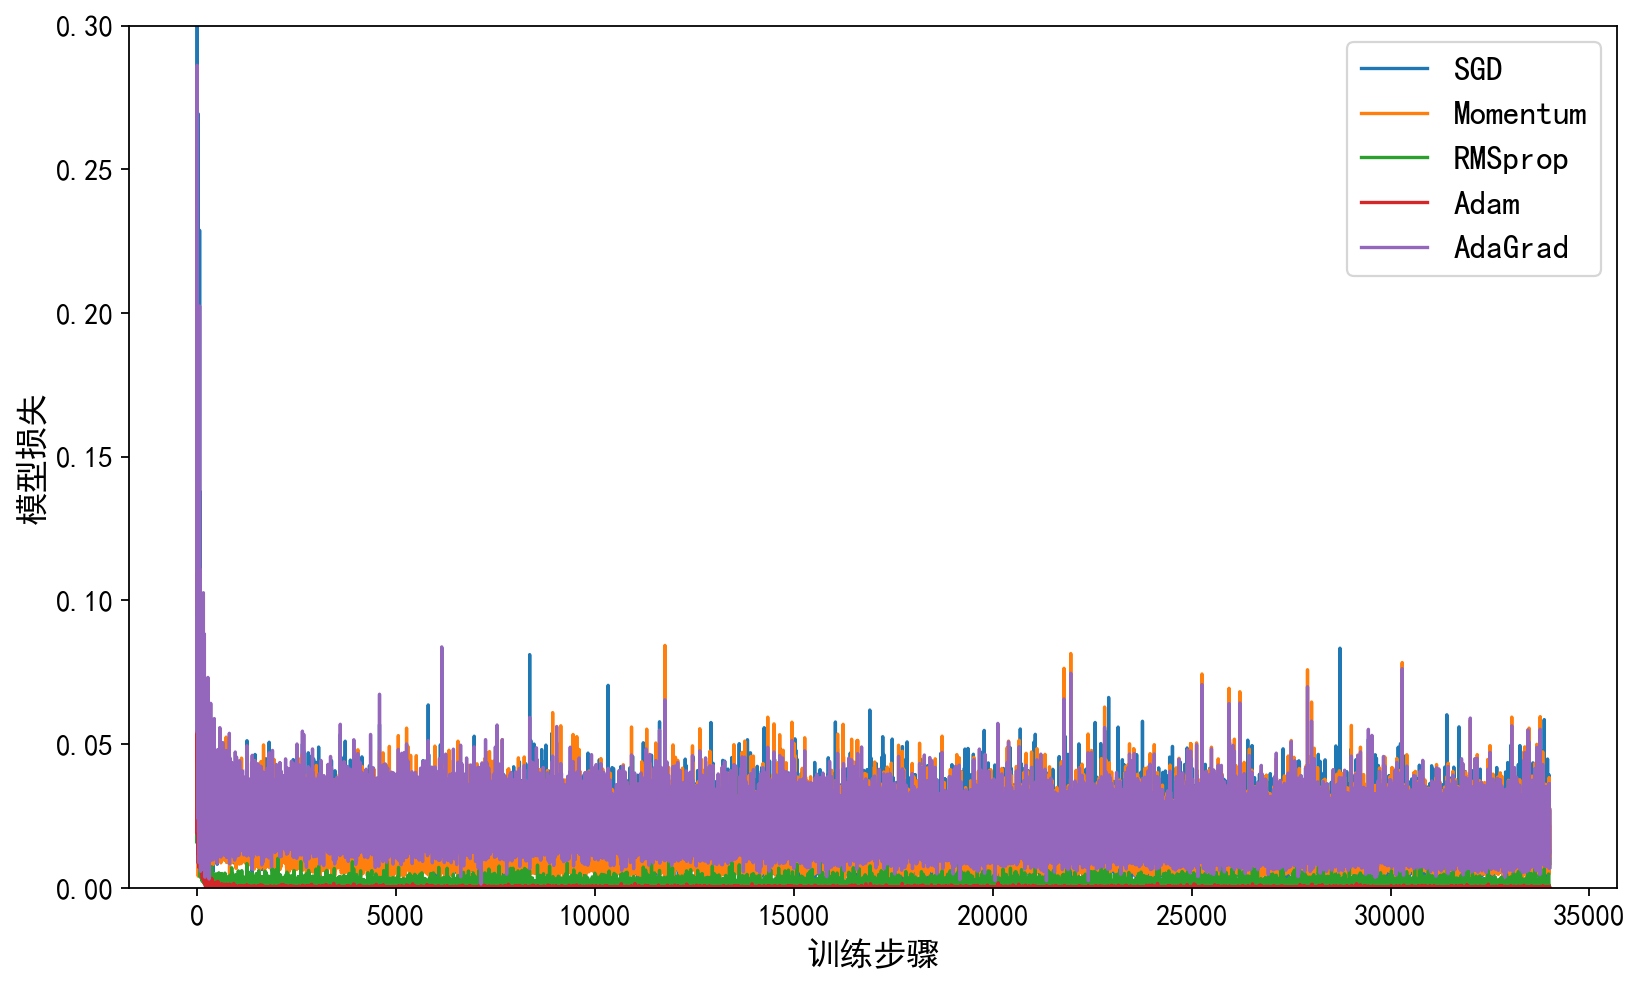
\includegraphics[width=0.6\textwidth]{part/人工智能/深度学习框架/pic/Pytorch/PyTorch神经网络工具/多种优化器比较.png}
    \caption{多种优化器比较}
    \label{fig:Pytorch_Multi_Optimizers_Comparison}
\end{figure}


\section{训练模型}
\label{subsec:Pytorch_train_model}
PyTorch训练模型主要包括加载数据集、损失计算、定义优化算法、反向传播、参数更新等主要步骤。
\subsection{加载和预处理数据集}
\label{subsubsec:Pytorch_load_and_preprocess_dataset}
可以使用PyTorch的数据处理工具，如\codeinline{torch.utils}和\codeinline{torchvision}等

\subsection{定义损失函数}
\label{subsubsec:Pytorch_define_loss_function}
可以通过自定义方法或使用PyTorch内置的损失函数定义损失函数，
如回归使用的\codeinline{loss\_fun=nn.MSELoss()},分类使用的\codeinline{nn.BCELoss}等损失函数


\subsection{定义优化方法}
\label{subsubsec:Pytorch_define_optimization_method}
PyTorch常用的优化方法都封装在\codeinline{torch.optim}中，
其设计很灵活，可以扩展为自定义的优化方法。

所有的优化方法都是继承了基类\codeinline{otim.Optimizer},并实现了自己的优化步骤。

如使用SGD优化器时，可设置\codeinline{optimizer = torch.optim.SGD(params,lr = 0.001)}。


\subsection{循环训练模型}
\label{subsubsec:Pytorch_loop_train_model}
\begin{enumerate}[label=\arabic*)]
    \item 设置为训练模式：
    调用\codeinline{model.train()}会把所有的module设置为训练模式。
    % \begin{lstlisting}[style=demostyle,numbers=none]
    % model.train()
    % \end{lstlisting}

    \item 梯度清零
    在默认情况下梯度是累加的，需要手工把梯度初始化或清零，调用\codeinline{optimizer.zero\_grad()}即可。

    \item 求损失值
    \begin{lstlisting}[style=demostyle,numbers=none]
    y_pred = model(x)
    loss = loss_fun(y_pred, y)
    \end{lstlisting}

    \item 反向传播(自动求导)
    调用\codeinline{loss.backward()}即可。

    \item 更新参数
    调用\codeinline{optimizer.step()}即可。
\end{enumerate}




\subsection{循环测试或验证模型}
\label{subsubsec:Pytorch_loop_test_or_validate_model}
\begin{enumerate}[label=\arabic*)]
    \item 设置为测试或验证模式：
    调用\codeinline{model.eval()}会把所有的\codeinline{training}属性设置为\codeinline{False}。

    \item 在不跟踪梯度的模式下计算损失值、预测值等
    \begin{lstlisting}[style=demostyle,numbers=none]
    with torch.no_grad():
        y_pred = model(x)
        loss = loss_fun(y_pred, y)
    \end{lstlisting}
\end{enumerate}

\subsubsection{比较model.train()和model.eval()的区别}
\label{subsubsubsec:Pytorch_compare_model_train_and_eval}
如果模型中有批量归一化(Batch Normalization, BH)层和dropout层，
需要在训练时添加\codeinline{model.train()},在测试时添加\codeinline{model.eval()}

其中\codeinline{model.train()}是保证BN层用每一批数据的均值和方差，
而\codeinline{model.eval()}是保证BN层用全部训练数据的均值和方差；

而对于dropout层,\codeinline{model.train()}是随机取一部分网络连接来训练更新参数，
而\codeinline{model.eval()}是利用所有网络连接。 

\subsection{可视化结果}
\label{subsubsec:Pytorch_visualize_results}

\section{正则化}
\label{subsec:Pytorch_regularization}
正则化是一种用于防止过拟合的技术，主要有L1正则化、L2正则化、Dropout等方法。
\subsection{L1正则化}
\label{subsubsec:Pytorch_L1_regularization}

\subsection{L2正则化}
\label{subsubsec:Pytorch_L2_regularization}

\subsection{Dropout}
\label{subsubsec:Pytorch_dropout}

\subsection{Batch Normalization}
\label{subsubsec:Pytorch_batch_normalization}

\section{训练技巧}
\label{subsec:Pytorch_training_techniques}


\section{保存和加载模型}
\label{subsec:Pytorch_save_and_load_model}
PyTorch中保存和加载模型的方法有多种，如保存和加载整个模型、保存和加载模型参数等。


\section{实例}
\label{subsec:Pytorch_nn_tools_example}
\subsection{模拟余弦函数曲线}
\label{subsubsec:Pytorch_simulate_cosine_curve}
\begin{lstlisting}[style=pythonstyle]
# 导入相关第三方库
import torch
import torch.nn as nn
from torch.utils.data import DataLoader
from torch.utils.data import TensorDataset
import numpy as np
import matplotlib
import matplotlib.pyplot as pit
matplotlib.rcParams['font.sans-serif'] = ['SimHei']
matplotlib.rcParams['axes.unicode_minus'] = False

# 准备拟合数据
x=np.linspace(-2*np.pi, 2*np.pi, 400)
y=np.cos(x)
X=np. expand_dims (x, axis=1)
Y=y.reshape(400,-1)
dataset=TensorDataset(torch.tensor(X,dtype=torch.float) , torch.tensor(Y,dtype=torch.float))
dataloader=DataLoader(dataset,batch_size=10,shuffle=True)

# 设置神经网络，这里就用一个简单的线性结构
class Net(nn.Module):
    def __init__(self):
        super(Net, self).__init__()
        self.net=nn.Sequential(
            nn.Linear(1,100),
            nn.ReLU(),
            nn.Linear(100,1)
        )
    def forward(self, input:torch.FloatTensor):
        return self.net(input)
    
net=Net()    

# 设置优化器和损失函数 
optim=torch.optim.Adam(Net.parameters(net),lr=0.001)
Loss=nn.MSELoss()

# 开始训练  
epochs=1000
for epoch in range(epochs):
    loss=None
    for batch_x, batch_y in dataloader:
        y_predict=net(batch_x)
        loss=Loss(y_predict, batch_y)
        optim.zero_grad()
        loss.backward()
        optim.step()
    if epoch%100==0:
        print(f'epoch:{epoch},loss:{loss.item()}')

predict=net(torch.tensor(X,dtype=torch.float))
# 可视化结果
pit.figure(figsize=(12, 7), dpi=160)
pit.plot(x, y, label="实际值", marker = "X")
pit.plot(x, predict.detach().numpy(), label="预测值", marker= 'o')
pit.xlabel("x", size=15)
pit.ylabel ("cos (x)", size=15)
pit.xticks(size=15)
pit.yticks(size=15)
pit.legend(fontsize=15)
pit.show()    
\end{lstlisting}
\begin{lstlisting}[style=demostyle,numbers=none]
epoch:0,loss:0.413939893245697
epoch:100,loss:0.005030750297009945
epoch:200,loss:0.0018504426116123796
epoch:300,loss:0.0018474120879545808
epoch:400,loss:0.0006889037904329598
epoch:500,loss:0.0005864549311809242
epoch:600,loss:0.0002862799447029829
epoch:700,loss:0.001682802801951766
epoch:800,loss:0.0007093378226272762
epoch:900,loss:3.737903170986101e-05
\end{lstlisting}    
\begin{figure}[htpb]
    \centering
    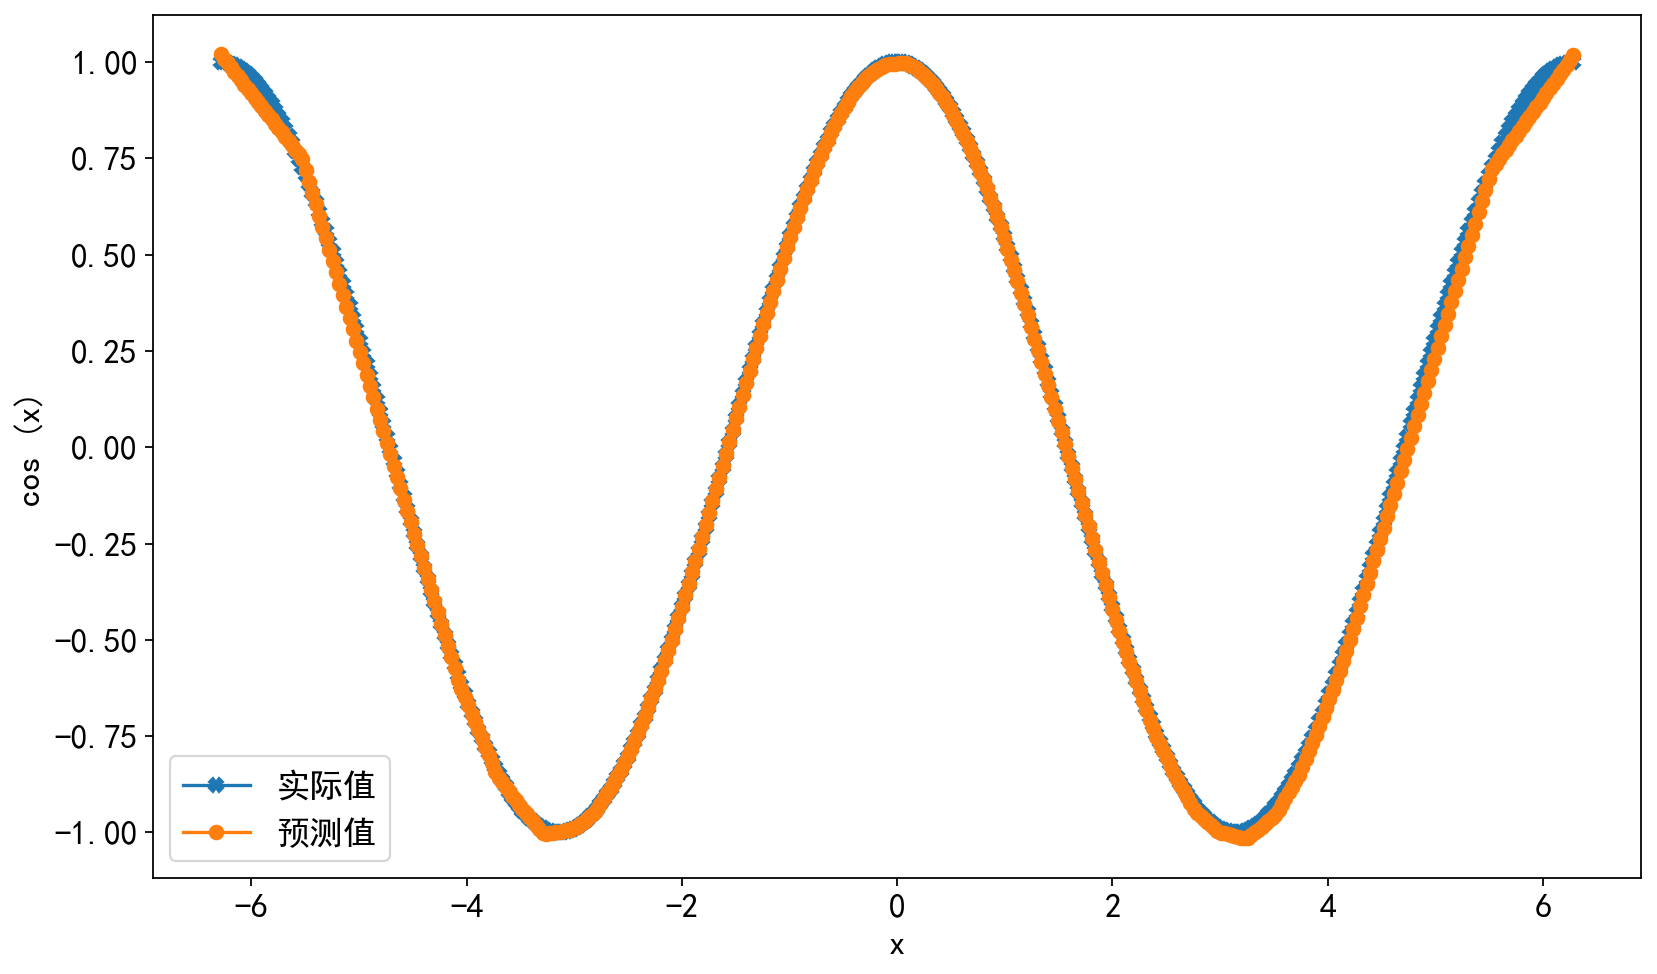
\includegraphics[width=0.6\textwidth]{part/人工智能/深度学习框架/pic/Pytorch/PyTorch神经网络工具/模拟余弦函数曲线.png}
    \caption{模拟余弦函数曲线}
    \label{fig:Pytorch_simulate_cosine_curve}
\end{figure}





